%!TEX root = ../thesis.tex
%*******************************************************************************
%******************************  5th  Chapter **********************************
%*******************************************************************************

\chapter{Experimental results}
\label{chap:xp}
% **************************** Define Graphics Path **************************
\ifpdf
    \graphicspath{{Chapter5/Figs/Raster/}{Chapter5/Figs/PDF/}{Chapter5/Figs/}}
\else
    \graphicspath{{Chapter5/Figs/Vector/}{Chapter5/Figs/}}
\fi



\section{Toy d'isabelle} % (fold)
\label{sec:toy_d_isabelle}

MNIST les 1 vs les 0.
Projection 1D.
L'observable est le nombre de pixel alumé et la systematique est la luminosité.
Ça donne une observable affectée par la systématique.

Mais si l'observable est la rondeur le l'image alors on a une observable orthogonale à la systématique.




\section{Technical difficulties} % (fold)
\label{sec:technical_difficulties}

Where do I write about the numerous issues ?
\begin{itemize}
  \item Inferno is unstable
  \item Pivot is unstable
  \item TP requires Jacobian vector product or takes crazy amount of time to train
  \item Regressor requires slow Adam and is probably a pain to train with gaussian mixture
  \item 
\end{itemize}



The benchmark is controlled with many parameters
\begin{itemize}
  \item Number of test samples
  \item Parameter of the toy model
  \item True value of the parameter of interest and nuisance parameters
  \item Sampling random seed
  \item TODO finish this list
\end{itemize}








\section{Performances on toys} % (fold)
\label{sec:performances_on_toys}

The idea is to do one subsection for one result 
\begin{itemize}
  \item Result 1 : The more test samples the better the inference
  \item Result 2 : Calib > Prior as expected
  \item Result final : Who is the best ? 
  \item 1. Baseline on nominal is as expected
  \item 2. All other methods on nominal also behave as expected
  \item 4. Regressor performances does not depend on the number of samples which is weird
  \item 5. Regressor estimated variance is probably broken
  \item 3. Asymetry with alpha because the problem itself is asymetric
\end{itemize}


Let's start with the results on the two toy problems (see \autoref{sec:toy_datasets} for details).
Toys provides a fully controled environement on various parameters of the problem to confront the proposed methods against different difficulties.
The first one is the small number of samples to do inference (\autoref{sub:performance_according_to_sample_size}).










\subsection{Performance according to sample size} % (fold)
\label{sub:performance_according_to_sample_size}

Here is summaried the performances measured according to the number of sample of the test set.



\victor{Performance en fonction du nombre d'events dans le dataset de test ? Evolution de la variance stat et syst en fonction de N\_samples.}


\begin{figure}[htb]
  \centering
  \begin{subfigure}[t]{0.49\linewidth}
    \includegraphics[width=\linewidth]{COMPARE/GG-prior/GradientBoostingModel/profusion_nominal_n_samples_mse.png}
    \caption{Gradient boosting}
    % \label{fig:gg-prior_GB_profusion_nominal_n_samples_mse}
  \end{subfigure}%
  \hfill
  \begin{subfigure}[t]{0.49\linewidth}
    \includegraphics[width=\linewidth]{COMPARE/GG-prior/NeuralNetClassifier/profusion_nominal_n_samples_mse.png}
    \caption{Neural network classifier}
    % \label{fig:gg-calib_best_average_errplot_mse}
  \end{subfigure}

  \begin{subfigure}[t]{0.49\linewidth}
    \includegraphics[width=\linewidth]{COMPARE/GG-prior/DataAugmentation/profusion_nominal_n_samples_mse.png}
    \caption{Data augmentation}
    % \label{fig:gg-prior_GB_profusion_nominal_n_samples_mse}
  \end{subfigure}%
  \hfill
  \begin{subfigure}[t]{0.49\linewidth}
    \includegraphics[width=\linewidth]{COMPARE/GG-prior/TangentPropClassifier/profusion_nominal_n_samples_mse.png}
    \caption{Tangent Prop}
    % \label{fig:gg-calib_best_average_errplot_mse}
  \end{subfigure}

  \begin{subfigure}[t]{0.49\linewidth}
    \includegraphics[width=\linewidth]{COMPARE/GG-prior/Inferno/profusion_nominal_n_samples_mse.png}
    \caption{Inferno}
    % \label{fig:gg-prior_GB_profusion_nominal_n_samples_mse}
  \end{subfigure}%
  \hfill
  \begin{subfigure}[t]{0.49\linewidth}
    \includegraphics[width=\linewidth]{COMPARE/GG-prior/Regressor/profusion_nominal_n_samples_mse.png}
    \caption{Regressor}
    % \label{fig:gg-calib_best_average_errplot_mse}
  \end{subfigure}


  \caption{MSE on nominal data for the baseline decrease as the number of samples increases.}
  \label{fig:gg_baseline_nominal_n_samples_mse}
\end{figure}













\subsection{Compare methods} % (fold)
\label{sub:compare_methods}


\begin{figure}[htb]
  \centering
  \begin{subfigure}[t]{0.49\linewidth}
    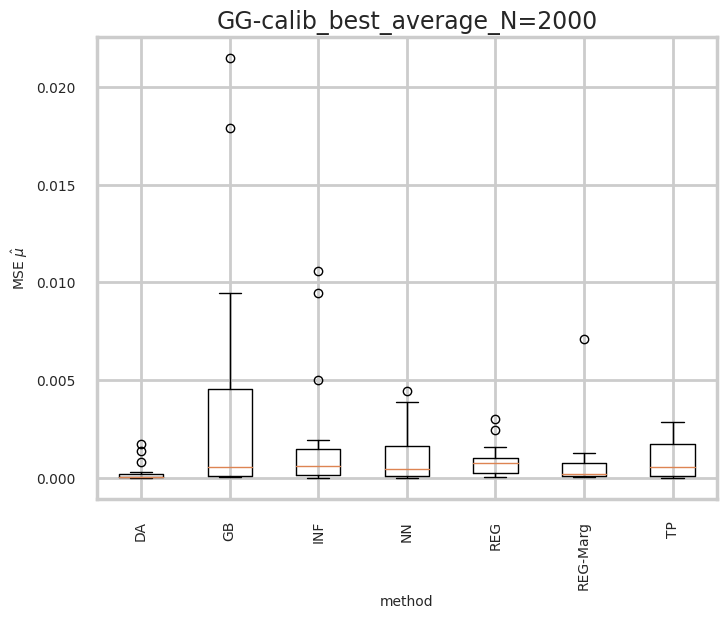
\includegraphics[width=\linewidth]{COMPARE/GG-calib/BEST_MSE/GG-calib_best_average_N=2000-boxplot_mse.png}
    \caption{boxplot of MSE}
    \label{fig:gg-calib_best_average_boxplot_mse}
  \end{subfigure}%
  \hfill
  \begin{subfigure}[t]{0.49\linewidth}
    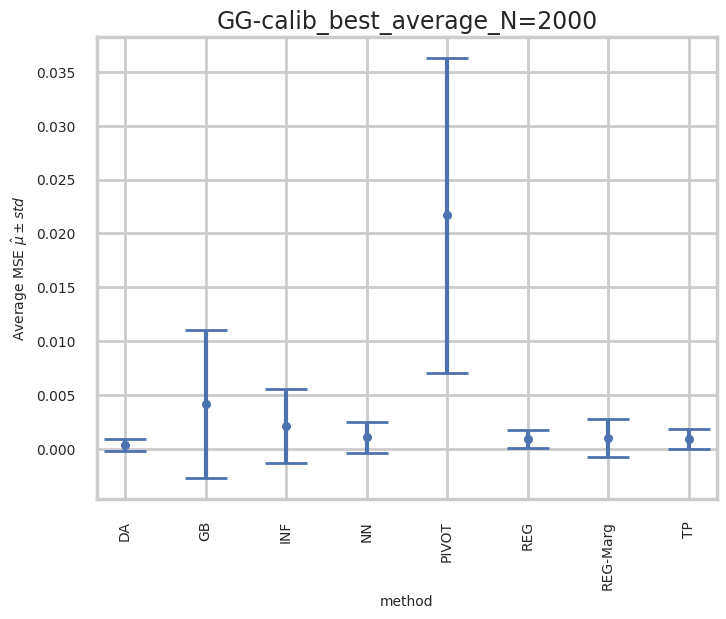
\includegraphics[width=\linewidth]{COMPARE/GG-calib/BEST_MSE/GG-calib_best_average_N=2000-errplot_mse.png}
    \caption{average MSE $\pm$ variance}
    \label{fig:gg-calib_best_average_errplot_mse}
  \end{subfigure}
  \caption{Best MSE on GG with 2000 test samples with calibration on data. Distribution according to $\mu^\star$ and $\alpha^\star$.}
  \label{fig:compare_gg_calib_best_mse}
\end{figure}











\subsection{Calibration influence} % (fold)
\label{sub:calibration_influence}

Then the best way to reduce the systematic uncertainty is to improve calibration !



\begin{figure}[htb]
  \centering
  \begin{subfigure}[t]{0.49\linewidth}
    \includegraphics[width=\linewidth]{COMPARE/GG-prior/NeuralNetClassifier/profusion_n_samples_mse.png}
    \caption{Prior calibration}
    % \label{fig:gg-prior_GB_profusion_nominal_n_samples_mse}
  \end{subfigure}%
  \hfill
  \begin{subfigure}[t]{0.49\linewidth}
    \includegraphics[width=\linewidth]{COMPARE/GG-calib/NeuralNetClassifier/profusion_n_samples_mse.png}
    \caption{Using data in calibration to infer $\alpha$}
    % \label{fig:gg-calib_best_average_errplot_mse}
  \end{subfigure}
  \caption{Calibration is the main influence on the inference.}
  \label{fig:gg_baseline_compare_calib_n_samples_mse}
\end{figure}


\begin{figure}[htb]
  \centering
  \begin{subfigure}[t]{0.49\linewidth}
    \includegraphics[width=\linewidth]{COMPARE/GG-prior/NeuralNetClassifier/profusion_true_mu_estimator.png}
    \caption{Prior calibration}
    % \label{fig:gg-prior_GB_profusion_nominal_n_samples_mse}
  \end{subfigure}%
  \hfill
  \begin{subfigure}[t]{0.49\linewidth}
    \includegraphics[width=\linewidth]{COMPARE/GG-calib/NeuralNetClassifier/profusion_true_mu_estimator.png}
    \caption{Using data in calibration to infer $\alpha$}
    % \label{fig:gg-calib_best_average_errplot_mse}
  \end{subfigure}
  \caption{Prior calibration leads to biased estimators.}
  \label{fig:gg_baseline_compare_calib_estimator}
\end{figure}

\victor{Biased estimator but I need to check the inference of $\alpha$ because it is a NLL with 2 minima !}







\section{Old stuff of chap 5} % (fold)
\label{sec:old_stuff_of_chap_5}


\begin{figure}[htb]
  \centering
  \begin{subfigure}[t]{0.49\linewidth}
    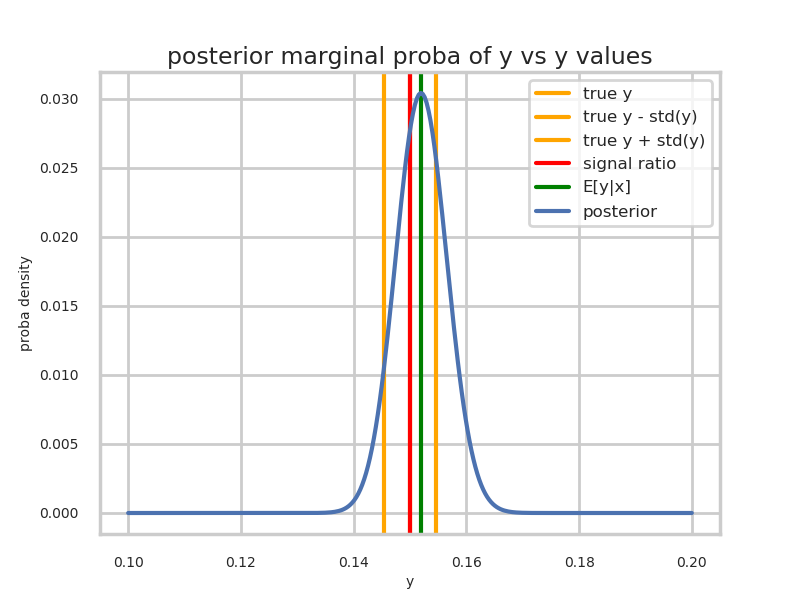
\includegraphics[width=\linewidth]{minitoy/marginal_y.png}
    \caption{$p(y|x)$}
    \label{fig:marginal_y}
  \end{subfigure}%
  \hfill
  \begin{subfigure}[t]{0.49\linewidth}
    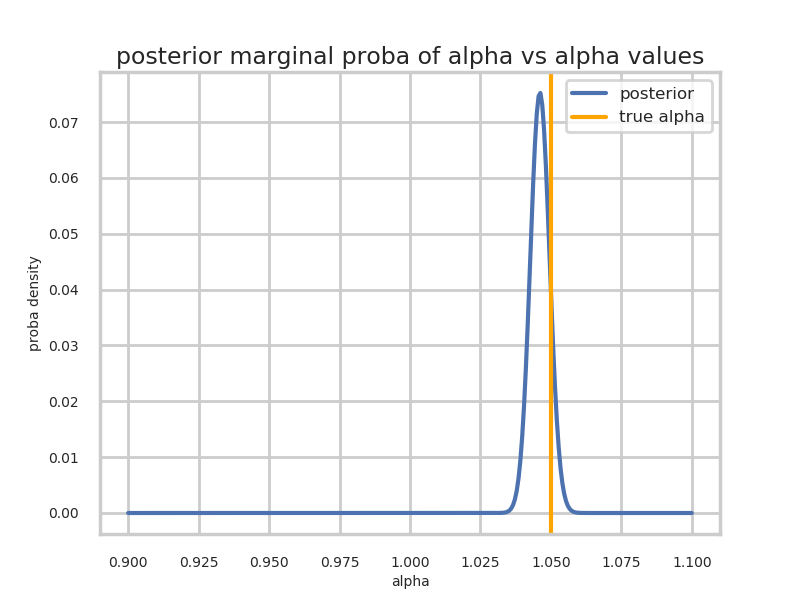
\includegraphics[width=\linewidth]{minitoy/marginal_alpha.png}
    \caption{$p(\alpha|x)$}
    \label{fig:marginal_alpha}
  \end{subfigure}
  \caption{Posterior probabilities for $y$ (left) and $\alpha$ (right)}
  \label{fig:marginals_gg}
\end{figure}

\emph{Remarque :}
L'erreur statistique et l'erreur systématique diminuent ensemble avec l'augmentation du nombre de donnée.
Plus on a de donnée meilleur est l'inférence sur $\alpha$.
Donc c'est normal !

Du coup j'ai vraiment du mal avec le concepte de l'erreur systématique qui ne diminue que doucement avec l'augmentation des données.

Si l'effet est invisible sur les données alors on a pas de problème.
Si l'effet est visible alors on peut contraindre + les paramètres de nuisance puisqu'on peut le mesurer !


\begin{figure}[htb]
  \centering
  \begin{subfigure}[t]{0.49\linewidth}
    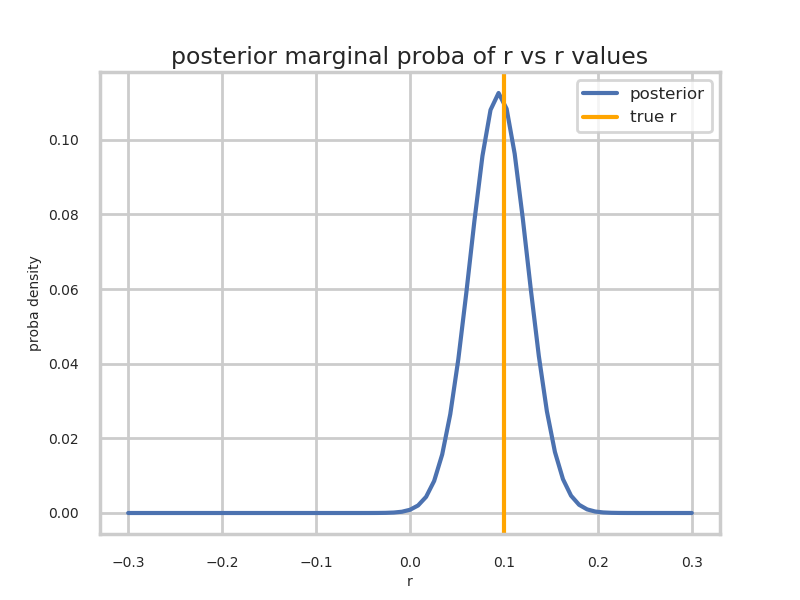
\includegraphics[width=\linewidth]{s3d2/marginal_r.png}
    \caption{$p(r|x)$}
    \label{fig:marginal_r}
  \end{subfigure}%
  \hfill
  \begin{subfigure}[t]{0.49\linewidth}
    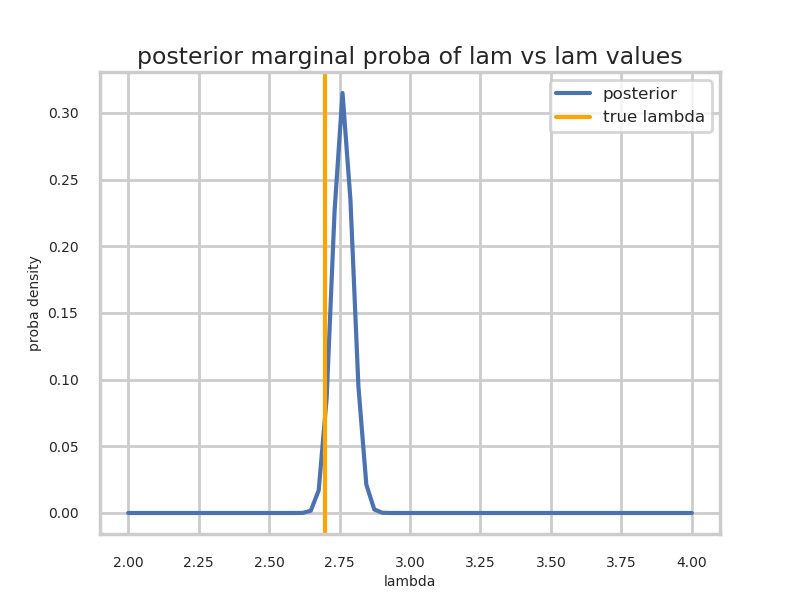
\includegraphics[width=\linewidth]{s3d2/marginal_lam.png}
    \caption{$p(\lambda|x)$}
    \label{fig:marginal_lambda}
  \end{subfigure}

  \begin{subfigure}[t]{0.49\linewidth}
    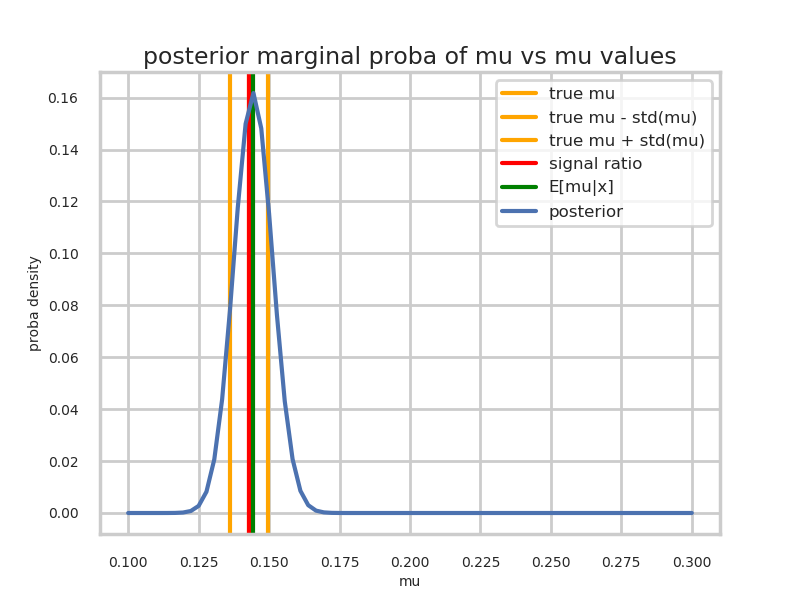
\includegraphics[width=\linewidth]{s3d2/marginal_mu.png}
    \caption{$p(\mu|x)$}
    \label{fig:marginal_mu}
  \end{subfigure}
  \caption{Posterior probabilities for $y$ (left) and $\alpha$ (right)}
  \label{fig:marginals_s3d2}
\end{figure}







\section{Real data} % (fold)
\label{sec:real_data}


\victor{Find out why this is does not work : \url{https://arxiv.org/pdf/1909.03081.pdf} ??}
\victor{La simulation est trop précise. cf resultat sur l'impossibilité de séparer les domaines créé}








\subsection{Nothing beats the baseline} % (fold)
\label{sub:nothing_beats_the_baseline}

\content{Show results on Higgs}







\subsection{Impossible to separate between domains} % (fold)
\label{sub:impossible_to_separate_between_domains}

\content{Show results of classifier trying to separate events between "extreme" values of nuisance params}









\subsection{Results with or without calibration} % (fold)
\label{sub:results_with_or_without_calibration}

\content{Compare results with or without using the current data in the calibration}







\subsection{Too rare signals} % (fold)
\label{sub:too_rare_signals}


\content{Explain and show that the issue comes from the imbalance between signals and backgrounds}

The scatter plot properties is much more dependent to noise or nuisance parameters than to the parameter of interest.




\section{Forest robustness} % (fold)
\label{sec:forest_robustness}

\victor{Grad boost is robust because trees disagrees between themselves}


